\noindent World is getting smaller every day, as new technologies constantly make communication and travelling faster and more effective then yesterday. Road network, Internet and many other networks are becoming more evolved and denser which also brings along new problems. In order to fully take advantage of such huge networks, we must have efficient algorithms that operate on these networks and give us answers to many questions. Among many others, one that we take particular interest in is the question: ``What is the shortest path from place $x$ to place $y$''?

In different networks, this question can make different sense. In the road network, we would like to obtain a sequence of intersections we have to go through in order to reach our destination, driving the shortest possible time (or the smallest possible distance). GPS devices and the likes of Google maps have to deal with this problem. In case of the Internet network, we might be interested in the shortest path to a destination computer in terms of router hops. In a network of social acquaintances, the smallest number of persons connecting us e.g. with guitarist Mark Knopfler or Liona Boyd could be expressed as a shortest path problem. Many problems in artificial intelligence (e.g. planning of actions) can be expressed, or include, looking for shortest paths.

\begin{wrapfigure}{r}{6cm}
	\centering
	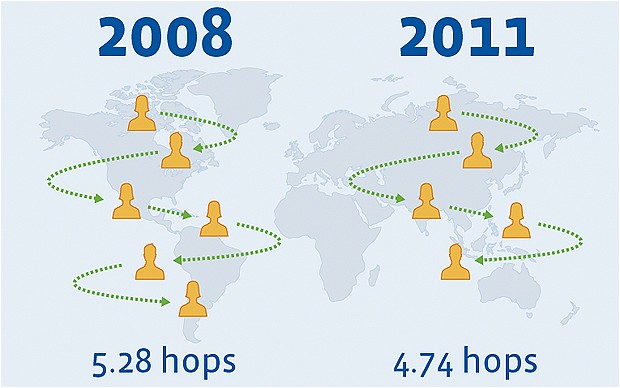
\includegraphics[width=5.5cm]{degrees.jpg}
	\caption{\label{fig:degrees} In a study carried out by Facebook it was claimed the average distance (in terms of friendship links) between the people on the site dropped from 5.28 in 2008 to 4.74 in 2011~\cite{degrees}.}
\end{wrapfigure}

The tremendous amount of work done in this area signifies the importance of quick distance or shortest path retrieval in graphs. A simple Dijkstra's or A* algorithm no longer comply to the requirements of today's applications, in which a server often has to answer hundreds of shortest path queries per second in a large-scale networks. To speed up the mentioned algorithms we usually sacrifice generality and concentrate on a particular type of network, or even on one concrete network.

In this thesis, the type of network we deal with is the one representing timetable connections, where nodes are the stations and arcs represent a direct connection between the two stations. We will talk in more details about this in following sections. However, this network has one substantial difference that we would like to point out - it is time-dependent. That means that the shortest path from station $x$ to station $y$ may have different solutions depending on the time when we start at station $x$. Therefore, we will not talk about shortest paths and distances, but rather about optimal connections and earliest arrivals and each query will now bear a third parameter - the departure time from $x$. \\

\noindent To informally develop the discussion about optimal connections in timetables, we will now clarify the motivation, approach and the goals of this thesis. We also sketch out the difference between the theory and practice when it comes to timetable search engines.

\subsection{Motivation}

	\noindent We have already approached the motivation in the introductory text. We consider that a server (hosting e.g. journey-planning application) has to answer many queries per given time unit. What does it mean many? British National Rails Enquiries website that hosts journey planner supports over 1 million queries per day~\cite{queriesnr}. Even if these queries were distributed evenly throughout the whole day, there would still be more than 11 queries per second. That is why the search engine run for each query has to be fast enough to provide an answer.
	
	11 queries per second is probably not a big issue. There is about 2500 railway stations in Great Britain and a current state of the art computer with basic implementation of a time-dependent Dijkstra's algorithm (to be talked about later) would be able handle the mentioned load without any problems. However, things get more difficult on a bigger scale, in rush hours and when additional requirements are posed on the search results (transfers, cost of travel or simply outputting more results the user can choose from).
	
	In shortest path routing on road networks very much has been done to speed-up the query times using pre-processing on the input graph (for a good review such methods, see~\cite{engineeringroute09}). Some developed methods answer distance queries more than 1 000 000 faster than the Dijkstra's algorithm on large road networks. In timetable scenario, the achieved speed-ups are much more modest. We will talk about the related work and achieved speed-ups in this area in the section~\ref{sec:relwrk}.
		
\subsection{Approach}

	\noindent We have mentioned that to get more effective algorithms with better query times, we need to focus on a special type of network and take advantage of its properties. In addition to this, what we can do is to pre-compute some information on the particular timetable and to use this information later to speed-up the answering of the queries. This is not a new technique and in the shortest path routing it is commonly referred to as creating distance oracle~\cite{apxdo05}. Our approach is analogical - instead of static graphs we deal with graphs representing the timetables~\footnote{Hence the name of this thesis - Distance oracles for timetable graphs, the ``distance'' being part of the title mostly because the term ``distance oracle'' is generally recognized.} and look for optimal connections. We will go more into the details about this approach in the preliminaries section~\ref{sec:prel}.
	
\subsection{Goals}
	
	\noindent We have set two main goals for this thesis:
	\begin{itemize}
		\item \textbf{Analyse real-world timetables} and their properties. More specifically, given the graph representing the timetable, we were interested in its sparsity, connectivity, average and maximal degrees, average optimal connection sizes... We will talk about these properties mostly in the section~\ref{sec:data}. 
		\item \textbf{Develop methods with fast query times} for optimal connections, based on pre-computing, as outlined in the previous subsection. For this purpose, we use also the outcomes of our analysis.
	\end{itemize}
	
\subsection{Theory and practice}

	\noindent This thesis is more theoretically oriented - we consider the optimal connection problem in probably its purest form, which does not account for the many requirements posed by travellers using timetable search engines. Those include number of transfers, preferred route, cost of travel and others. These multi-criteria queries are discussed e.g. in~\cite{timetablemodelsalgs07}. In practice, we also usually want to output multiple connections, so that the user has a chance to choose. Needless to say, all of this makes the problem much more complicated and challenging than a pure search for an optimal connection.
	
	On the other hand, the real-world timetable search engines concentrate usually on one given dataset, which enables them to exploit its properties~\footnote{E.g. An the city of Bratislava has only four (functioning) bridges, which could be taken into account when designing a public transportation search engine.} and tailor the search engine specifically for it. There is also a choice of a suitable timetable model based on the characteristics of the given timetable.
	
	The aim of the theoretical works (like this thesis) is not therefore to develop an algorithm immediately deployable into practice but rather to investigate techniques which might be useful to consider when designing practical timetable search engines.
	
\subsection{Organization \& conventions}

	\noindent This thesis is organized as follows: 
	\begin{itemize}
		\item \textbf{Preliminaries}: We provide the necessary definitions (most notably timetable and its graph representations) and formally define the problem we deal with, as well as the approach we use
		\item \textbf{Related work}: This section summarizes the main related work in distance oracles, static route-planning and time-dependent scenarios
		\item \textbf{Data \& analysis}: We introduce real-world timetables we worked with and analyse many of their properties
		\item \textbf{Underlying shortest paths}: In the main part of the thesis, we present the two methods we developed to speed-up optimal connection queries in timetables. These methods are also analysed from both theoretical and practical point of view
		\item \textbf{Neural network approach}: We summarize a little experiment in which we tried to train neural network to answer optimal connection queries
		\item \textbf{Application TTBlazer}: This section shortly describes the application we used to analyse our datasets and test the methods
		\item \textbf{Conclusion}: Finally, we conclude pointing out main results and contribution, drawbacks and possibilities for future work
	\end{itemize}
	\hspace{\fill}
	
	\noindent In this thesis, we also use some conventions:
	\begin{itemize}
		\item With a few exceptions, we will use \textbf{bold} font to mark currently defined term (or its notation)
		\item Names of our algorithms are in \textit{italics}
	\end{itemize}
	